\documentclass[a4paper, 11pt]{article}

\usepackage{hyperref} % Provides the \url{} command
\usepackage{graphicx} % Provides the \includegraphics[]{} command

\setlength{\parindent}{3ex} % Set indent length

\begin{document}

\title{A Comparative Analysis of Constituencies in England and Wales}
\author{{\small\textsc{Dan Saattrup Nielsen}}}
\date{\today}
\maketitle

\abstract{
  {\footnotesize We will perform a cluster analysis of constituencies in England and Wales, based on population, area, average age, median house price, amount of businesses, business profile, qualifications and presence of various amenities. This allows us to find similar areas in England and Wales given any specified location in England and Wales.}
}


\section{Introduction}
One of the decisions growing businesses have to make is which city they would like to expand to. Which cities have the most similar characteristics to enable a business potential?

The current project provides a first attempt at a solution to the above, by grouping similar cities in the UK based on population, area, average age, median house price, amount of businesses, business profile, qualifications and presence of various amenities.

Aside from the abovementioned use case we could imagine this analysis also being useful for other purposes. For instance, advertisement companies would be able to advertise more cost-efficiently, rather than paying large sums for nationwide advertisements.


\section{Data}
All our data used are both free and publicly available and have been downloaded from the Office of National Statistics (\url{www.ons.gov.uk}). Links to these can conveniently be found at the Constituency Dashboard
\begin{center}
  \url{commonslibrary.parliament.uk/local-data/constituency-dashboard/}
\end{center}

The specific data sets that we used were the following:
\begin{enumerate}
  \item Median house prices by constituency, 2013
  \item Number of VAT and/or PAYE based enterprises by constituency, 2018
  \item Population and age distribution by constituency, 2017
  \item Qualifications by constituency, 2011
  \item Area in hectar by constituency, 2015
\end{enumerate}

We will also be using a data set on constituencies and their latitudes and longitudes from \url{www.doogal.co.uk}, as well as using their API to fetch constituency information of a given location. Lastly, we will use the Foursquare API to get data regarding amenities present in the constituencies.

The house price and population data sets only covered England and Wales. It was possible to find population information from the Scottish government's website, but house price information is only provided by Scottish constituency, which is a completely different layout compared to the Westminster Parliamentary Constituencies that we are using. We therefore opted to stick with only England and Wales, as the data in those countries are uniform.
 

\section{Methodology}
We decided to give equal weight onto our eight variables:
\begin{enumerate}
  \item {\tt pop}, the total population
  \item {\tt area}, the area in hectars
  \item {\tt avg\_age}, the average age
  \item {\tt house\_price}, the median house price
  \item {\tt business}, the total amount of businesses
  \item {\tt business\_profile}, the distribution of businesses by sector
  \item {\tt quals}, the distribution of the level 1--4 qualifications
  \item {\tt amenity}, the frequency of about 400 types of amenities\\
\end{enumerate}

To be able to achieve this, we would have to derive a single number from each variable, for each constituency. Achieving this for {\tt pop}, {\tt area}, {\tt avg\_age}, {\tt house\_price} and {\tt business} were straightforward: we simply gathered the respective values and normalised them.

As for the {\tt business\_profile}, {\tt quals} and {\tt amenity}, these variables are multidimensional, so to deal with this problem we used a Principal Component Analysis on these three variables to reduce them down to a one-dimensional variable. We lose some data as we are doing this, but this seems more desirable than letting these multi-dimensional variables dominate the clustering. After having reduced them down to one dimension we subsequently normalised them.

\begin{figure}
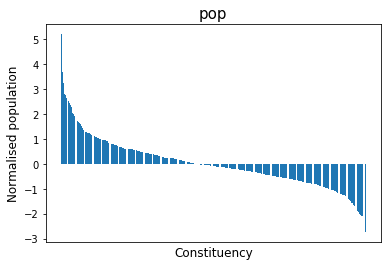
\includegraphics[scale=.43]{../gfx/pop.png}
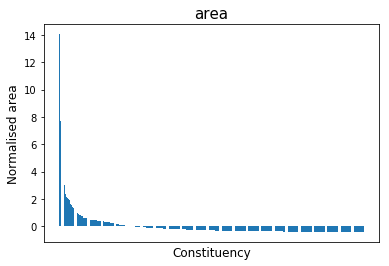
\includegraphics[scale=.43]{../gfx/area.png}\\
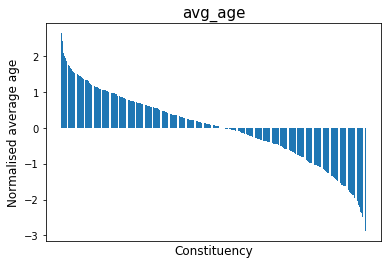
\includegraphics[scale=.43]{../gfx/avg_age.png}
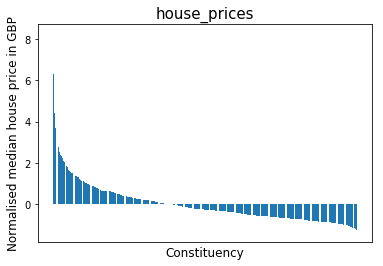
\includegraphics[scale=.43]{../gfx/house_price.png}\\
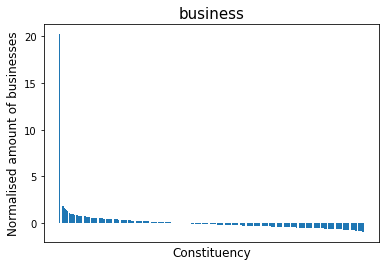
\includegraphics[scale=.43]{../gfx/business.png}
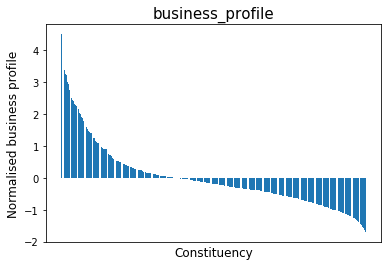
\includegraphics[scale=.43]{../gfx/business_profile.png}\\
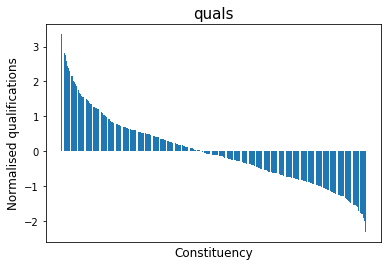
\includegraphics[scale=.43]{../gfx/quals.png}
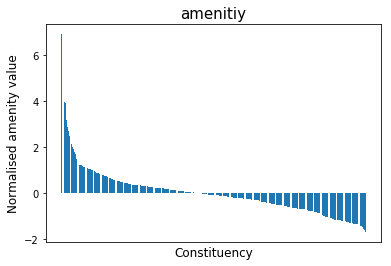
\includegraphics[scale=.43]{../gfx/amenity.png}
\caption{Normalised distributions of variables.}
\end{figure}

We wanted to include as many relevant variables as possible, to ensure that we can (meaningfully) distinguish between most constitencies. We can ``track'' our progress here by the following scatter plots of the successively merged variables, reduced down to two dimensions using Principal Component Analysis solely to enable visualisation.

\begin{figure}
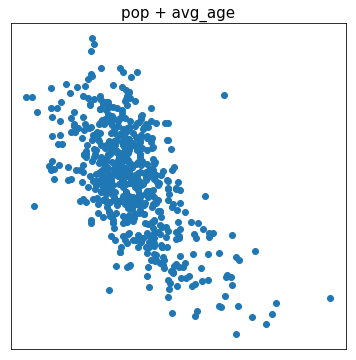
\includegraphics[scale=.32]{../gfx/cluster0.png}
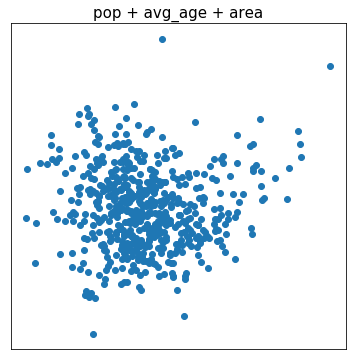
\includegraphics[scale=.32]{../gfx/cluster1.png}
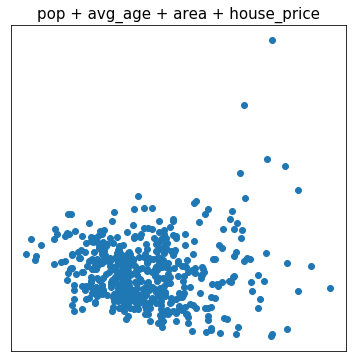
\includegraphics[scale=.32]{../gfx/cluster2.png}\\
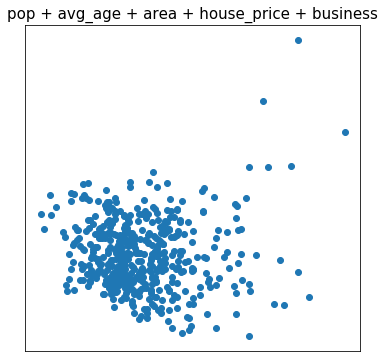
\includegraphics[scale=.32]{../gfx/cluster3.png}
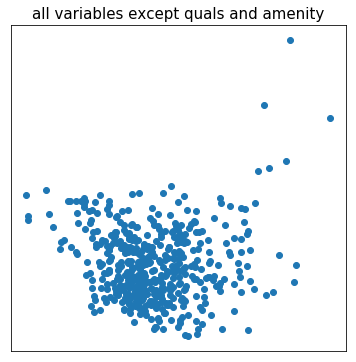
\includegraphics[scale=.32]{../gfx/cluster4.png}
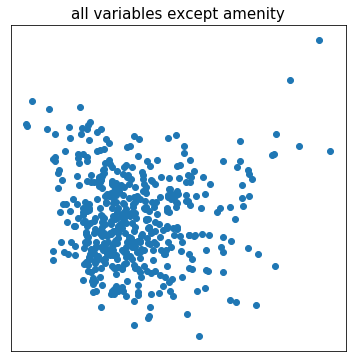
\includegraphics[scale=.32]{../gfx/cluster5.png}\\
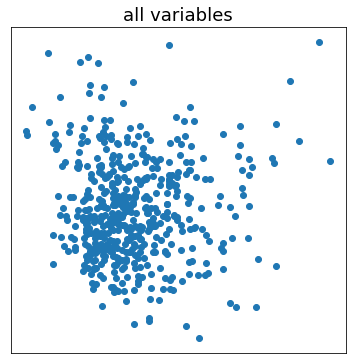
\includegraphics[scale=.32]{../gfx/cluster6.png}
\caption{Successive distributions of constituencies.}
\end{figure}

We decided to use the k-means clustering algorithm to group the constituencies together. We opted to not go with a density-based clustering algorithm like DBSCAN as our data is focused around a single large cluster, and so such an algorithm would group together too many constituencies that are not like each other. To find the optimal k we started by performing the ``elbow method''.

\begin{center}
  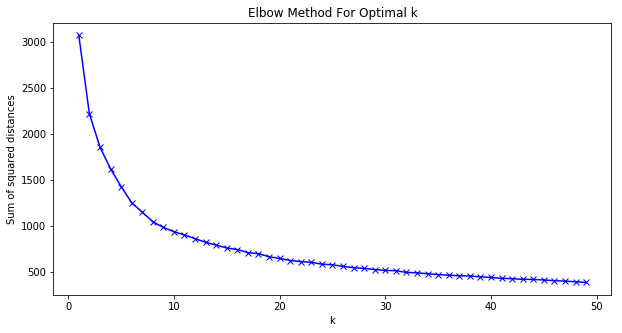
\includegraphics[scale=.5]{../gfx/elbow0.png}
\end{center}

We see here that the elbow is when k=8. With this choice of k our cluster distribution looks like the following.

\begin{center}
  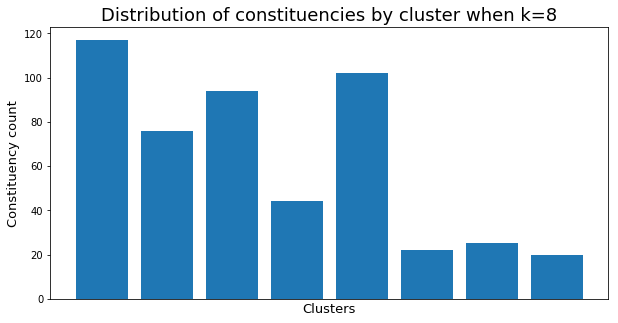
\includegraphics[scale=.4]{../gfx/cluster_dist0.png}
\end{center}

When it comes to our particular use case, narrowing all constituencies down to fewer than 50 is great, but narrowing it down to 100-175 does not provide that much value. Therefore we try to look for the second ``elbow'' occuring after k=8.

\begin{center}
  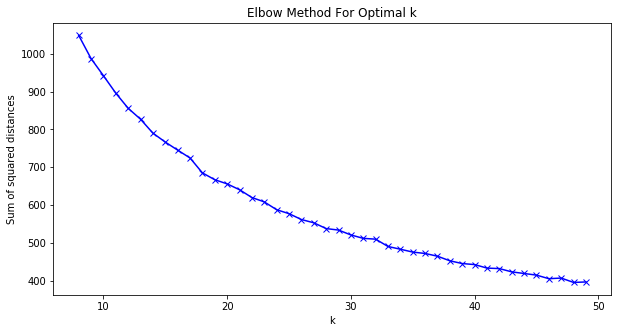
\includegraphics[scale=.5]{../gfx/elbow1.png}
\end{center}

The ``elbow'' here are not as clear as previously, but we \textit{do} see that the slope decreases at k=18. The cluster distributions for this k-value is as follows.

\begin{center}
  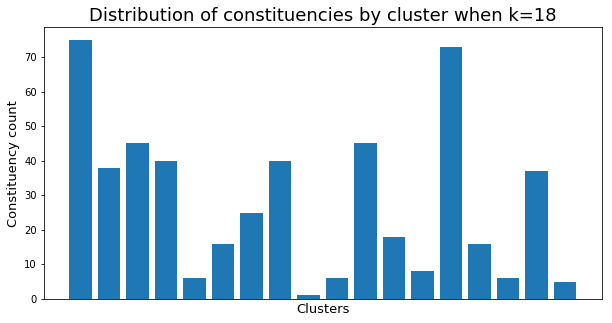
\includegraphics[scale=.4]{../gfx/cluster_dist1.png}
\end{center}

Purely based on our use case we will therefore use k=18. We are aware that by not using k=8 we will risk artifically separating similar constituencies, and a more in-depth analysis is needed to determine whether such a choice of k above 8 can be meaningfully assigned.

\section{Results}
We have applied a k-means clustering algorithm to our eight variables to group constituencies in England and Wales. We end up with the following clustering, where we keep in mind that the clustering lives in eight dimensions and constituencies that appear to be close to each other in the following plot might be more separated.

\begin{center}
  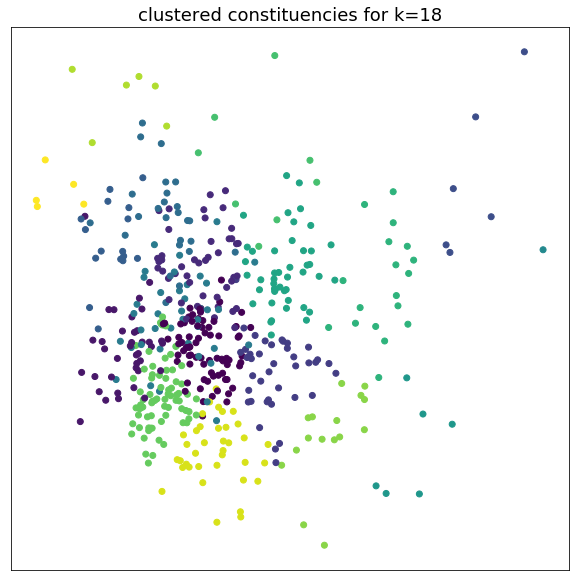
\includegraphics[scale=.40]{../gfx/cluster_colour.png}
\end{center}

Now, using this clustering, we can then find similar areas to a specified location as follows. From the location we first find a list of the nearby postcodes, using the \url{doogal.co.uk} API, and we then find the constituency in which the nearest postcode is located, which is also found using the \url{doogal.co.uk} API.

\qquad Next, we find the cluster in which the constituency belongs to and display a map of all the constituencies in this cluster. For instance, inserting the location ``Bristol'' we are presented with the following map.

\begin{center}
  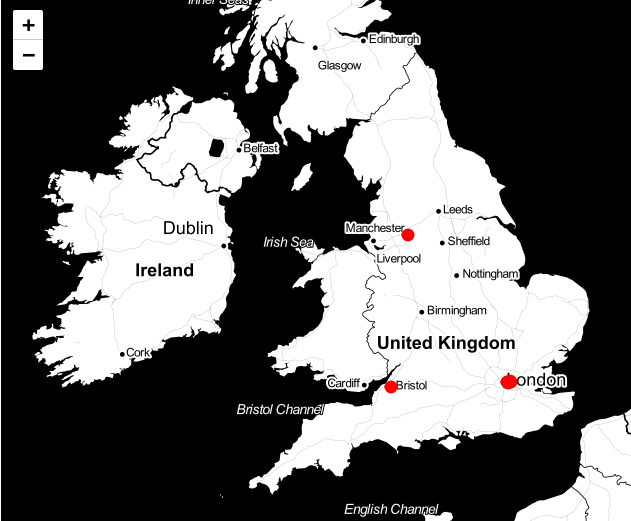
\includegraphics[scale=.40]{../gfx/map0.png}
\end{center}

The cluster shown here is comprised of the following constituencies:
\begin{itemize}
  \item Bristol West
  \item Manchester Central
  \item Bethnal Green and Bow, London
  \item Poplar and Limehouse, London
  \item West Ham, London
  \item East Ham, London\\
\end{itemize}

We get the following map by inserting the location ``Swansea'':

\begin{center}
  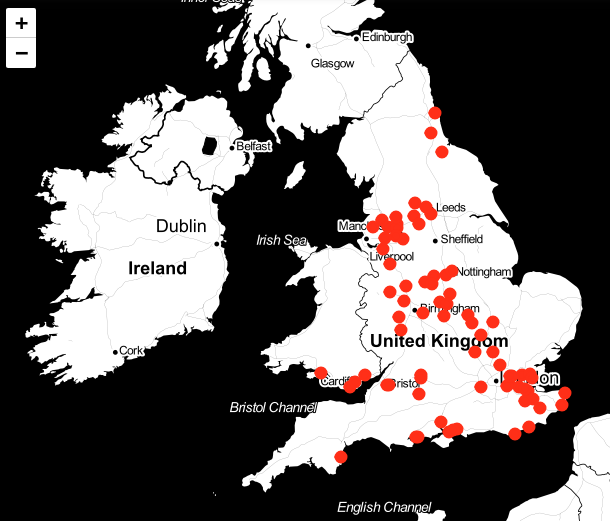
\includegraphics[scale=.40]{../gfx/map1.png}
\end{center}

Here we see that Swansea shares a lot of commonalities between many coastal areas in the south as well as several places in eastern London, the midlands and around Manchester and Leeds. Notably, it does not include any city centres.


\section{Discussion}
This is an initial clustering of the constituencies in England and Wales, and has by no means been perfected in any way. Further work would need to be done to find significant reasons for the choice of a particular k in the k-means clustering algorithm, as varying k will produce quite different results. Several of the data sets did not include all the constituencies in England and Wales, which also excluded some potential similar areas as well as not working for the excluded areas. Including all constituencies would then be a mixture of gathering more data and possibly applying classification algorithms to fill in missing values.

However, that being said, the model \textit{does} produce a list of similar areas to the given input, which significantly reduces the amount of areas that a company would need to analyse.


\section{Conclusion}
We have gathered data from five different data sets and from the Foursquare API and aggregated the information into eight normalised variables. We next performed a k-means clustering on these variables, which can then be used to find similar locations in England and Wales based on any location given in England or Wales. This can be valuable to a company that want to branch out to other similar areas, as it provides suggestions as to what areas they might want to consider, rather than them checking through all 500+ constituencies or relying on gut feeling. 


\end{document}
